%%%%%%%%%%%%%%%%%%%%%%%%%%%%%%%%%%%%%%%%%%%%%%%%%%%%%%%%%%%%%%%%%%%%
% Grundlagen
%%%%%%%%%%%%%%%%%%%%%%%%%%%%%%%%%%%%%%%%%%%%%%%%%%%%%%%%%%%%%%%%%%%%

\chapter{Preliminaries}
  \label{PR}
This chapter introduces terms and definitions used in this thesis. \autoref{basics} explains what a graph is in graph theory and what attributes a graph can have. 
\autoref{LL} gives an introduction to linear layouts and distinguishes the different characteristic of linear layouts.
\autoref{SAT} provides the reader with a short explanation of SAT. 
\section{Basics}
\label{basics}
Formally a graph $G = (V, E)$ consists of a finite set of vertices $V$ and a finite set of edges $E \subseteq V \times V$, where each edge $e_i$ connects two vertices $v_j, v_k \in V$. We state that $n := |V|$ and $m := |E|$.\\
A \textit{path} $p$ is a series of edges $(e_1, e_2,...,e_m), e_1,...,e_m \in E$. The same path can also be described as a sequence of vertices $(v_1,v_2,...,v_k)$, where for example $e_1$ connects $v_1$ to $v_2$.
\subsection{Attributes of a graph}
\subsubsection{Directed or undirected}
A graph can be either \textit{directed} or \textit{undirected}.\\
In a \textit{directed} graph all edges $e \in E$ are described as ordered pairs of vertices $e = (u,v)$, where the first vertex is referred to the source and the second is referred to as the target vertex.\\
In an \textit{undirected} graph each edge is defined by an unordered pair of vertices $e = {u,v}$ with no definite source or target. 
\subsubsection{Weighted or unweighted}
A graph can have \textit{weighted} or \textit{unweighted} edges.\\
If a graph is \textit{weighted} its definition includes a transformation $w: E \rightarrow \mathbb{R}$ which assigns a weight to each edge $e \in E$. 
\subsubsection{Complete} 
A \textit{complete} graph contains an edge $e$ for every pair of vertices $v, u \in V$. \textit{Complete} graphs are denoted as $K_n$ where $n = |V|$.\\
A \textit{directed} complete graph with $n$ vertices has exactly $n^2$ edges, whereas an \textit{undirected} complete graph has only $\frac{n^2 -n}{2}$ edges. The complete graphs $K_4$ and $K_5$ can be seen in \autoref{PPG}.
\subsubsection{Connected}
A graph is called \textit{connected}, if for every two vertices $v_i, v_j \in V$ there is a path from $v_i$ to $v_j$, meaning there are no unreachable vertices (see in \autoref{img:COAC}a, where vertex 5 is unreachable).
\subsubsection{Acyclic}
An \textit{acyclic} graph has no cycles, which means that there exists no path $(v_0, v_1,...,v_k)$ where $v_0 = v_k$, that is to say that for every path in the graph the start vertex and end vertex can not be the same (see in \autoref{img:COAC}).
\begin{figure}[h!]
\begin{center}
\includegraphics[width= \textwidth]{figures/ConnectedAcyclic.png}
\caption{Connectivity and acyclicity: a) neither connected nor acyclic graph b) connected and acyclic graph}
\label{img:COAC}
\end{center}
\end{figure}
\subsubsection{Bipartite}
A graph is called \textit{bipartite} if its vertices $V$ can be divided in two disjoint subsets $V_0, V_1 \subset V$ such that $V_0 \cup V_1 = V$, and each edge $(u,v) \in E$ connects one vertex from $V_0$ with one vertex from $V_1$ (see in \autoref{BTF}).\\
\subsubsection{Trees and forests}
A \textit{tree} is a \textit{connected}, \textit{acyclic} graph.\\
A \textit{forest} is an graph consisting of several tree graphs, meaning it is not \textit{connected} but still \textit{acyclic}.
\begin{figure}[h!]
\begin{center}
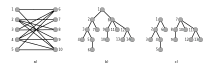
\includegraphics[width= \textwidth]{figures/BipartiteTreeForest.png}
\caption{Different graphs a) A bipartite graph, b) a tree, c) a forest}
\label{BTF}
\end{center}
\end{figure}

\subsubsection{Planar}
A graph is \textit{planar} if it can be drawn in a two dimensional plane such that no two edges $e_i, e_j \in E$ cross (see \autoref{img:crossNest}) \\
A graph is \textit{maximal planar} if no edge can be added to the graph without loosing the planarity. $K_4$ is the biggest \textit{complete} graph that is planar.\\
The drawing of a graph is referred to as \textit{plane} if no edges cross. Note that a graph can be \textit{planar} but a particular embedding of the graph is not necessarily \textit{plane}.
\begin{figure}[h!]
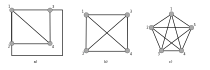
\includegraphics[width =\textwidth]{figures/PlanarPlaneGraphs.png}
\caption{On planarity a) $K_4$, planar graph and plane drawing, b) $K_4$, planar graph but not plane drawing, c) $K_5$, neither planar graph nor plane drawing}
\label{PPG}
\end{figure}\\
The \textit{plane} drawing of a \textit{planar} graph can be divided into certain areas which are called faces. The inner faces of a graph are areas enclosed by edges. The outer face of graph is infinitely large and means the area outside the graph, bounded by its outer edges.
\newpage
\section{Linear layouts}
\label{LL}
%\cite{dujmovic2004linear}
A linear layout of a graph is a layout in which all the vertices $V$ are positioned along a line called the \textit{spine}.\\
The order in which these vertices are placed on the spine, is described by a bijective function $$\sigma : V \mapsto \{1,...,n\} $$ This function defines a relation where the following statements hold:
\begin{itemize}
\item Antisymmetry: if $\sigma(v_0) \leq \sigma(v_1)$ and $\sigma(v_1) \leq \sigma(v_1)$ then $v_0 = v_1$
\item Transitivity: if $\sigma(v_0) \leq \sigma(v_1)$ and $\sigma(v_1) \leq \sigma(v_2)$ then $\sigma(v_0) \leq \sigma(v_2)$
\item Connexity: either $\sigma(v_0) \leq \sigma(v_1)$ or $\sigma(v_1) \leq \sigma(v_1)$ is true
\end{itemize}
These properties make the relation a \textit{total order} and the set of vertices a \textit{linearly ordered set}.\\
The edges of the graph are sorted into $p$ disjoint subsets $E_p \subseteq E$ by the surjective function 
$$ \pi: E \rightarrow \{1,..,p\} $$ making it a partition of $E$.\\
In the linear layout each subset represents one half-plane, delimited by the spine, on which all the edges will be placed.
In order to make it possible to draw these graphs in a 2D setting the edges of a half-plane are often colored which is why the half planes are sometimes also referred to as \textit{colors}.\\
The following sections explain which requirements the order of vertices and the assignment of edges follow.
\begin{figure}[!h]
\begin{center}
\includegraphics[width=1\textwidth]{figures/CrossingNesting.png}
\caption{Edges a) crossing edges, b) nesting edges}
\label{img:crossNest}
\end{center}
\end{figure}
\subsection{Stack layouts}
For a stack layout $\mathcal{E}(G,p)$, sometimes also referred to as a \textit{book embedding}, the vertices $V$ need to be ordered in a way that now two edges $e_i, e_j$ assigned to the same subset $\pi(e_i) = \pi(e_j)$ cross (see \autoref{img:crossNest}), that is to say each each half plane contains a \textit{planar} subgraph. The subsets $E_p$ in a stack layout are calles \textit{pages} or \textit{stacks}.\\
The \textit{book thickness} or \textit{stack number} of a graph defines the minimal number of pages that is needed to embed the graph.\\
In 1986 Prof. Dr. Mihalis Yannakakis \cite{yannakakis1986four} was able to prove that every planar graph admits to a stack layout with $p \leq 4$. Prof. Yannakakis also sketched the construction of a graph whose book thickness $p = 4$. However, his sketch was never completed and to this day researchers have not been able to find a graph that requires four pages (see further explanation in \autoref{Exp}).
\begin{figure}[!h]
\begin{center}
\includegraphics[width=0.7\textwidth]{figures/K4Stack.png}
\caption{$K_4$ and the corresponding stack layout}
\label{img:stackGHG}
\end{center}
\end{figure}
\subsection{Queue layouts}
For a queue layout $\mathcal{Q}(G,q)$ the order of the vertices is chosen such that no two edges $e_i, e_j$ on the same pages are nested. Two edges $e_i, e_j$ are nested if both endpoints of edge $e_i$ are between both endpoints of edge $e_j$ (see \autoref{img:crossNest}). This property is not violated if edges $e_i, e_j$ share the same source or target vertex.\\
Similar to the \textit{book thickness} in stack layouts a queue layout has a \textit{queue number} that states in how many queues the graph can be embedded in minimally.\\
The upper bound for the queue number of planar graphs is $\mathcal{O}(log^4 n)$ \cite{di2013queue}.
\begin{figure}[!h]
\begin{center}
\includegraphics[width=0.7\textwidth]{figures/K4Queue.png}
\caption{$K_4$ and the corresponding queue layout}
\label{img:queueK4}
\end{center}
\end{figure}
\subsection{Further restrictions}
In addition to either being a stack or a queue, each half plane can be restricted further to have a special graph structure.
\subsubsection{Tree or forest subgraphs}
A half plane or page of the layout has to be in the structure of a \textit{tree} or \textit{forest}, meaning that it is \textit{acyclic} and in the case of a \textit{tree} also connected.
\subsubsection{Dispersable subgraphs}
A \textit{dispersable} subgraph is a graph in which no two edges share one endpoint. This kind of graph is also called a \textit{matching} \cite{kaufmann2018dispersable}. 
\begin{figure}[h!]
\begin{center}
\includegraphics[width=1\textwidth]{figures/ForestDisp.png}
\caption{A linear layout with one forest stack (red) and one dispersable stack (blue)}
\label{img:plzhltr}
\end{center}
\end{figure} 
\section{SAT}
\label{SAT}
In 2015 the Algorithms Research Group of University of Tübingen proposed a new method to compute linear layouts automatically \cite{Bekos2015TheBE}, by formulating the problems as an instance of SAT which can then be solved in reasonable time.\\
A logical formula for SAT is in \textit{conjunctive normal form}, that means it is a conjunction (and, $\land$) of clauses or literals, and the clauses are disjunctions (or, $\lor$) of literals.\\
SAT-Solver usually use a nondeterministic algorithm, that means for the same instance it can return different solution.\\
For a detailed explanation of this refer to \cite{Bekos2015TheBE, jess}. The translation of the graph to a SAT instance is executed on \url{http://sofa.fsi.uni-tuebingen.de:5555/}.
